
\begin{figure}[h]
\centering
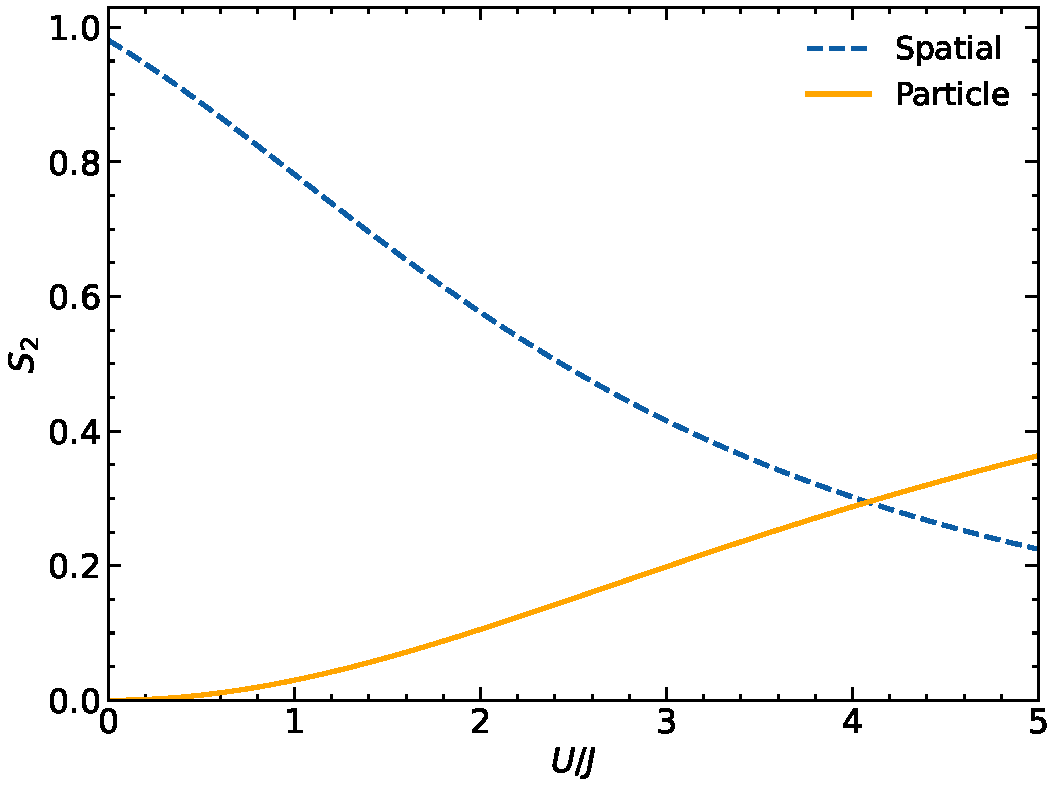
\includegraphics[scale=0.5]{../figures/ed_renyi.pdf}
\caption{The figure above is a graph of the Renyi entanglement entropy for both spatial and particle bipartitions versus the ratio of the interaction term to the hopping term.}
\end{figure}

\subsection{PIGSFLI Algorithm}

A Monte Carlo simulation is a stochastic (random) method of integration, which allows for accurate estimations of desired values. Monte Carlo is necessary for situations where exact calculations are too computationally expensive, such as in the exact diagonalization of the reduced density matrix for high particle/site number Bose Hubbard systems. The size of the Hilbert space is calculated by \cref{eq:36} and shown by \cref{fig:hilbert_space_size}:

\begin{equation}
D = \frac{\left(N+L-1\right)!}{\left(N\right)!\left(L-1\right)!}
\label{eq:36}
\end{equation}

\begin{figure}[h]
\centering
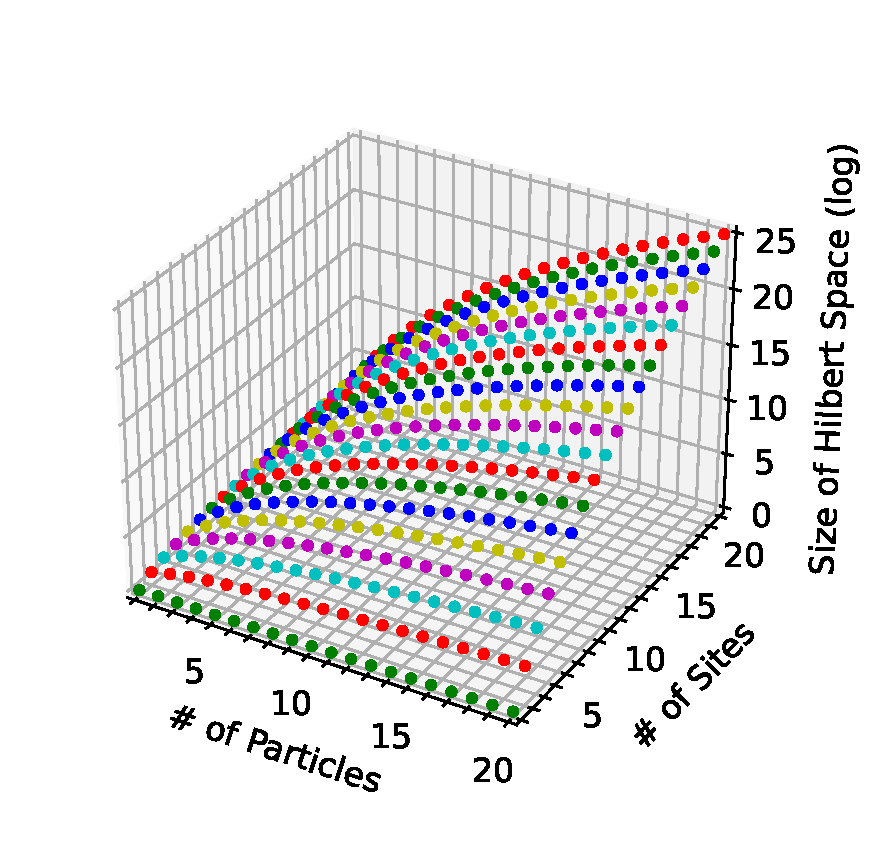
\includegraphics[scale=0.5]{../figures/hilbert_space_size.pdf}
\caption{The figure above shows the size of the Hilbert space as a function of number of sites and particles. This 3-dimensional plot for the number of combinations in the Hilbert space goes up to $20$ sites and $20$ particles.}
\label{fig:hilbert_space_size}
\end{figure}
